\documentclass[a4paper,12pt]{scrartcl}

\usepackage[utf8]{inputenc}

%\usepackage[latin1]{inputenc}
\usepackage{amsfonts}
\usepackage{amsmath}
\usepackage{amssymb}
\usepackage{amsthm}
\usepackage{color}
\usepackage[ngerman]{babel}
\usepackage[pdftex]{graphicx}
%\usepackage[T1]{fontenc}
\usepackage{graphics,color} 
\usepackage{graphicx}
\pagestyle{empty}
\usepackage{float}
%\topmargin20mm
\oddsidemargin0mm
\parindent0mm
\parskip2mm
\textheight25.5cm
\textwidth15.8cm
\unitlength1mm

\newcommand{\E}{\mathbb{E}}
\newcommand{\Hy}{\mathbb{H}}
\newcommand{\N}{\mathbb{N}}
\newcommand{\RR}{\mathbb{R}}
\newcommand{\Z}{\mathbb{Z}}
\newcommand{\Q}{\mathbb{Q}}
\newcommand{\C}{\mathbb{C}}
\newcommand{\K}{\mathbb{K}}
\newcommand*\ee{\mathrm{e}}
\newcommand*\ii{\mathrm{i}}
\newcommand*\re{\mathrm{Re}}
\newcommand*\im{\mathrm{Im}}
\newcommand*\id{\mathrm{id}}
\newcommand*\glnr{\mathrm{\it GL}(n,\R)}
\newcommand*\slnr{\mathrm{\it SL}(n,\R)}
\newcommand*\on{\mathrm{\it O}(n)}
\newcommand*\son{\mathrm{\it SO}(n)}
\newcommand*\rang{\mathrm{Rang}}
\newcommand*\grad{\mathrm{grad~}}
\newcommand*\dive{\mathrm{div~}}
\newcommand*\sym{\mathrm{Sym}}
\newcommand*\spur{\mathrm{Spur}}
\newcommand*\isom{\mathrm{Isom}}
\newcommand*\bmo{{\bf o}}
\newcommand*\bmu{{\bf u}}
\newcommand*\bmw{{\bf w}}
\newcommand*\bmx{{\bf x}}
\newcommand*\bmb{{\bf b}}
\newcommand*\bmc{{\bf c}}
\newcommand*\bmy{{\bf y}}
\newcommand*\bma{{\bf a}}
\newcommand*\bmp{{\bf p}}
\newcommand*\bmm{{\bf m}}
\newcommand{\cls}{\color{blue}}


%\author{Gabriele Link}

\begin{document}


%\vspace*{-20mm}
% \vspace*{-35mm}  %FUER pdflatex

%\begin{picture}(4,2)
% Die folgenden 2 Zeilen sind als Kommentar zu 
% kennzeichnen, falls kein Logo gewuenscht
%\put(0,0){
%\includegraphics[width=4cm]{kit_logo_de_farbig.jpg}}
%\end{picture}\hfill

%\hspace{9cm}


\section*{\large Einf\"uhrung in die Computergrafik \\\vspace*{5mm}
                  \normalsize  Aufgabenblatt 2 }
\hrule
\hrule
\vspace{4mm}
%\includegraphics[width=0.8\textwidth]{sampleplot.pdf}

{\bf Aufgabe 1. Polygonale Netze \hfill (4 Punkte)}

Schreiben Sie ein Programm/Methode  namens planeMesh(int a, int b, int ma, int mb ) in Pseudocode, welches  das folgendes leistet:
\begin{itemize}
\item Als Eingabe werden Integer  int a, int b, int  ma und int mb akzeptiert.
\item Ausgabe ist ein Netz im Datenformat der Eckenliste eines Ebenen-Abschnittes, das durch Dreiecke entsprechend der Skizze modelliert wird.
\item Der Ebenenabschnitt beginnt in $\begin{pmatrix} 0 \\ 0 \\ 0\end{pmatrix}$ und breitet sich dann in $x$-Richtung bis $\begin{pmatrix} a \\ 0 \\ 0\end{pmatrix}$ aus und in  $y$-Richtung bis $\begin{pmatrix} 0 \\ b \\ 0\end{pmatrix}$. 
\item Die Zwischenpunkte haben jeweils den abstand $a/ma$ in $x-Richtung$ und $b/mb$ in $y$-Richtung.
 \end{itemize}

\begin{figure}[H]
    \centering
    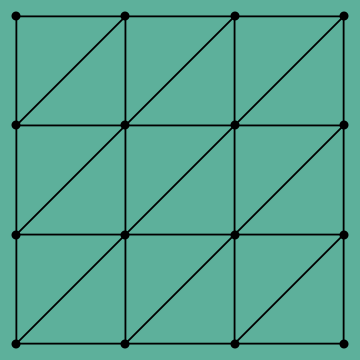
\includegraphics[width=0.4\textwidth]{plane.png}
    
\end{figure}

\vspace*{4mm}




{\bf Aufgabe 2. Binomialkoeffizient. \hfill (4 Punkte)}

Beweisen Sie (durch vollständige Induktion), dass  der Binomialkoffizienten für alle $n \in \mathbb{N}$ die Rekursionsformel  
\begin{align*}
\begin{pmatrix} n \\ i \end{pmatrix} = \begin{pmatrix} n-1 \\ i \end{pmatrix} + \begin{pmatrix} n-1 \\ i-1 \end{pmatrix}  \; .
\end{align*}
erfüllt.
\vspace*{8mm}


\newpage 

{\bf Aufgabe 3. Bezierkurven. \hfill (4 Punkte)}

Zeigen Sie, dass eine Bezierkurve   $B^n(t) := \sum_{i = 0}^{n} B_i^n(t) \cdot  b_i$  die Ableitung
\begin{align*}
(B^n)'(t) = n \cdot \sum_{j = 0}^{n-1} B_{j}^{n-1}(t) \cdot (b_{j+1} - b_j) 
\end{align*}
 hat.


\vspace*{4mm}

{\bf Aufgabe 4.  Der Algorithmus von de Casteljau. \hfill (4 Punkte)}

Sei $B^n(t) := \sum_{i = 0}^{n} B_i^n(t) \cdot  b_i$ eine Bezierkurve mit den Kontrollpunkten $b_i \in \mathbb{A}^3$.
Beweisen Sie den Algorithmus von de Caseljau, also dass
 $b_n^n = B^n(t_0)$ für alle $t_0 \in [0,1]$ gilt, wobei
\begin{align*}
b_i^k := \begin{cases}
b_i   & i= 0, \hdots,  n \\
(1-t_0) \cdot b_{i-1}^{k-1} + t_0 \cdot b_{i}^{k-1} &  i = 1, \hdots , n \; \;   k = 1, \hdots , i 
\end{cases} 
\end{align*}
rekursiv definiert ist.

 





\vfill

\hrule
{\bf Abgabe} der L\"osungen  bis  {\bf Freitag}, den 27.11.2015.  

\end{document}
